
\section{Implementation in Virtual Wall}
\label{sec:impl-vw}
% In this section, the implementation is introduced indicating the testbeds involved in it and the required steps for the implementation.

% Fistly, the implementation of the \sss in \vw is depicted. The designed topology and the new
% modified topology (different to the designed one) are depicted because of the handicaps of
% the hardware during the implementation. Then, nodes reservation is
% explained and detailed. Finally, the scripts included in each type of
% node are described before the presentation of the execution.

% The next section is dedicated to the implementation of the software
% developed in the \bonfire testbed. Nodes reservation is firstly
% depicted. Architecture and setup are also explained. And again, the
% scripts for each node setup are included before the description of the
% execution.

% Finally, the integration between \vw and \bonfire is described.

% Section 6 is devoted\ to\ describe the\ demonstration\ of the\ GEO-Cloud
% experiment prepared for the European Commission in June 2014.

In this section, the implementation of the \sss in \vw is explained. First, the designed
topology and the new modified topology (different to the design one) are layed out because
the handicaps of the hardware during the implementation. Then, nodes reservation is
explained and detailed. Finally, the scripts included in each type of node are described
before the presentation of the execution.


% \bigskip

% Finally, section 7 provides\ the main\ conclusions.


\subsection{Topology network}

The \sss is comprised of the
following modules:
\begin{itemize}
\item The \emph{Satellite System Simulator}
\item The \emph{Ground Station System Simulator}
\end{itemize}
The topology network designed is depicted in Figure~\ref{fig:impl-topology-vw}.

\begin{figure}[!h]
\hspace{-1cm}
\begin{center}
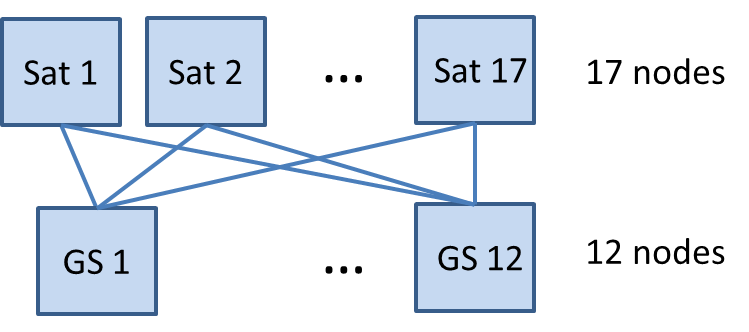
\includegraphics[width=0.68\textwidth]{implementationVWBF/gs-sat.png}

\caption{Topology Network in \vw}
\label{fig:impl-topology-vw}
\end{center}
\end{figure}



The previous topology network involves Sat nodes to have 12 connections with the GS nodes; and GS nodes 17 connections with Sat nodes plus one connection with the \bonfire cloud.

The nodes in \vw have a limitation of 5 physical connections. To deploy the previous
topology we adapted the \sss software to establish those connections by software. This was
done by making the \satss flexible to connect with any ground station from GS1 to GS12. 

The solution was to multiply the \satss by 3 and connect 4 ground stations to each \satss. This ensures the same performance and dynamics of the previous topology network described in Figure~\ref{fig:impl-topology-vw}, and the only thing it changes is the software.

The \sss implemented in \vw is depicted in Figure~\ref{fig:impl-nodes-vw}.

\begin{figure}[!h]
\begin{center}
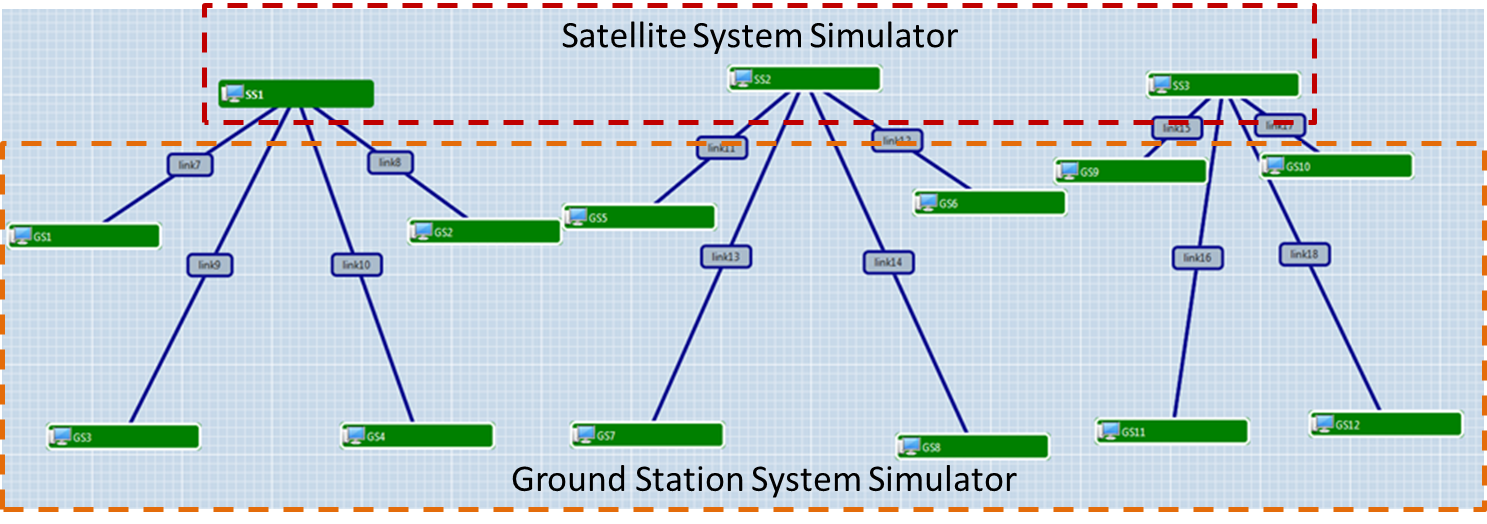
\includegraphics[width=0.9\textwidth]{implementationVWBF/nodes-vw.png}

\caption{Topology Network of the \satss}
\label{fig:impl-nodes-vw}
\end{center}
\end{figure}



\subsubsection{Nodes Reservation and Setup}

The \sss is then constituted by 15 ``Generic nodes'' in \vw 1 (The \vw
testbed is composed by two sets of machines, \vw 1 and \vw 2). The configuration of the experiment makes the provisioning of ``any available node'',
which is more flexible in case a node is being used in other experiment (see Figure~\ref{fig:creating-node-jfed}). The links between SS \emph{(Satellite Simulators)} and GS \emph{(Ground Stations Simulators)} nodes
are \ac{TCP}. The definition of the dependencies and the commands that will be installed at
setup is defined in \emph{JFed} using a \emph{Rspec} specification. This specification includes some
bash commands or instructions that will execute after reservation automatically.


\begin{figure}[!h]
\begin{center}
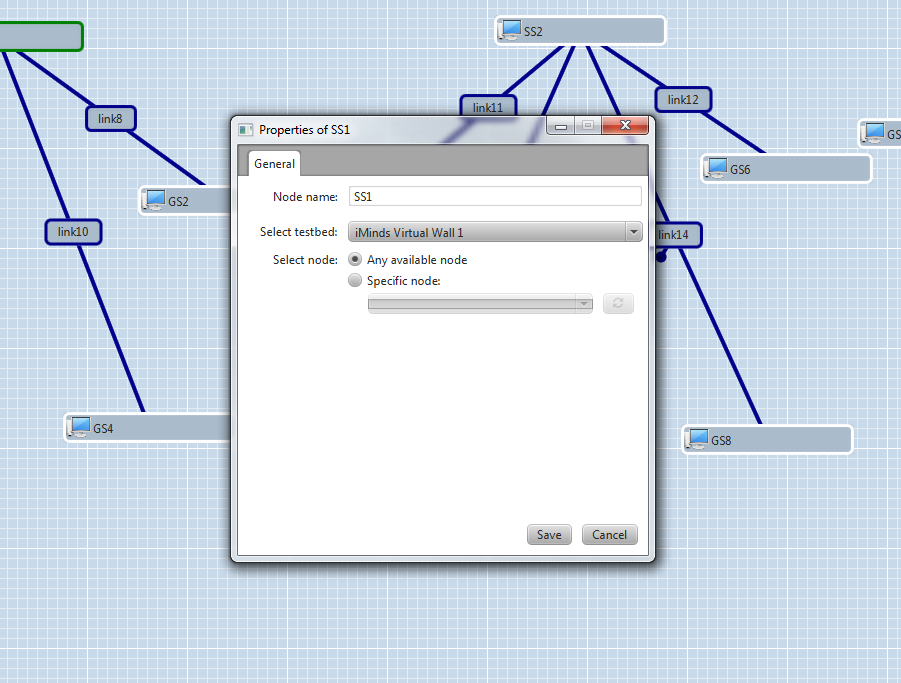
\includegraphics[width=0.9\textwidth]{implementationVWBF/creating-node-jfed.png}

\caption{Configuration of \vw nodes}
\label{fig:creating-node-jfed}
\end{center}
\end{figure}


\paragraph{Satellite Simulator Nodes Setup}~\\
The configuration of the nodes is done by using \emph{JFed Rspec Experiment}. The
setup steps are the following:
\begin{itemize}
\item To configurate a gateway for obtaining Internet connectivity and installing the
  needed libraries.
\item To update the system.
\item Once the update is finished, dependencies can be installed.
\item As the simulators require a connection with a database, the \emph{MySQL} library is
  also required. 
\item Source is downloaded from Google Drive where is located.
\end{itemize}

The script that perform the above is showed in Listing~\ref{code:impl-rspec-sat-sim}.

\lstset{float=h!,caption={Rspec specification for \emph{Satellite Simulators}},style=customc,numbers=left,label={code:impl-rspec-sat-sim}}
\lstinputlisting[firstline=2,lastline=14]{../../source/vw/Description.rspec}



Where <<google\_drive\_host\_address>> is the address of the Google Drive URI in which the scripts are located.

The \emph{Database} is located in \bonfire and it has an \emph{IP address} that can change. In order to
obtain that \emph{IP address} and include it in the \emph{Satellite Simulator}, a simple script to
acquire the \emph{IP address} of the database was developed \emph{push\_dbIP.sh}.
Listing~\ref{code:impl-script-ipdb} contains the script.

\lstset{float=h!,caption={Bash script to write the Database's \emph{IP address} on a file},style=customc,numbers=left,label= code:impl-script-ipdb}
\lstinputlisting{../../source/vw/push_ip.sh}

The execution of the \emph{push\_dbIP.sh} script acquires the \emph{IP address} of the database and includes it in the file \emph{ipdb}, created by \emph{push\_dbIP.sh}.
Finally, the node is perfectly configured to proceed with the installation of the
\emph{Satellite Simulator}. The software of the simulator has been archived too in
\emph{Google Drive}. The software is acquired and it can now be executed in the node.


\subsubsection{Ground Station Simulator Nodes Setup}


The \emph{Ground Station Simulators} software is developed under Python. The steps of
setup are the following:
\begin{itemize}
\item To configurate a gateway for obtaining Internet connectivity and installing the
  needed libraries.
\item To update the system.
\item Once the update is finished, dependencies can be installed.As occurred with the SS nodes, the update and the installation of Python and MySQL are required.
\item As the simulators require a connection with a database, the \emph{MySQL} library is
  also required. 
\item Source is downloaded from Google Drive where is located.
\item The database IP address is added to \emph{ipdb} file.
\item  The raw data is located in Google Drive too.  
\item The GS nodes are required to open an \emph{FTP} to be accessed from the
\emph{Orchestrator} in \bonfire. The \emph{FTP} is configured by executing the
\emph{install\_ftp.sh} file. This file content is in Listing~\ref{code:impl-ftp-installation}.  
\end{itemize}

The script that perform the above is showed in Listing~\ref{code:impl-rspec-gs-sim}.

\lstset{float=h!,caption={Rspec specification for \emph{Ground Station Simulators}},style=customc,numbers=left,label={code:impl-rspec-gs-sim}}
\lstinputlisting[firstline=64,lastline=78]{../../source/vw/Description.rspec}


\lstset{float=h!,caption={FTP server installation},style=customc,numbers=left,label={code:impl-ftp-installation}}
\lstinputlisting{../../source/vw/install_ftp.sh}


Through the FTP connection the raw data will be transferred from the GS nodes to the BonFIRE cloud. 

The execution of the Satellite Simulators and the Ground Station Simulators are described
in Section~\ref{par:sat-simulator-execution} and Section~\ref{par:sss-ground-execution}. 

% Local Variables:
%   coding: utf-8
%   fill-column: 90
%   mode: flyspell
%   ispell-local-dictionary: "american"
%   mode: latex
%   TeX-master: "main"
% End:
